% !TeX root = ../main.tex
\section{Iteratives Vorgehen zur Lösung linearer Gleichungssysteme}
\subsection{Splittingverfahren}
Gegeben sei das LGS $Ax=b$ für $A\in\mathbb{K}^{n\times n}, b\in\mathbb{K}^n, x\in\mathbb{K}^n$, 
wobei $\mathbb{K}\in\{\mathbb{R}, \mathbb{C}\}$. Wir wollen dieses LGS nun in ein FP-Problem umformen, 
sei hierfür $A$ nicht singulär (sonst nicht lösbar). \\
Wir schreiben $A=M-N$, wobei $M$ invertierbar und häufig sogar eine Diagonalmatrix ist 
(damit $M$ leicht zu invertieren ist). Dies liefert:
\[Ax = b \Leftrightarrow (M-N)x=b \Leftrightarrow Mx=Nx+b x=\underbrace{M^{-1}\cdot(Nx+b)}_{\Tilde{T}x}\]
$\Tilde{T}$ ist affin-linear. Wir erhalten also unser FP-Problem $x=\Tilde{T}x=Tx+c$ 
mit $T=M^{-1}N$ und $c=M^{-1}b$ \\ \\

\algobox{Splittingverfahren}{
\begin{algorithm}[H]
    \SetAlgoNoLine
    \InitTe{$A=M-N$ mit $N\in GL(n,\mathbb{K})$}{}
    \SetAlgoLined
    Wähle $x^{(0)}\in\mathbb{K}^n$ beliebig \\
    \ForTe{$k=0,1,\dotsc$}{
        löse $Mx^k=Nx^{k-1}+b$} 
    \SetAlgoNoLine
    \UntilTe{stop (beliebiges Stopkriterium)}{}
\end{algorithm}
}
Konvergenz dieses Algorithmus folgt aus Banachschen Fixpunktsatz.

\begin{rembox}
    Nach gleicher Überlegung lässt sich auch unser obiges Splittingverfahren für Nullstellenbestimmung herleiten:
    \[f(x)=0\Leftrightarrow h(x)+g(x):=f(x) = 0 \Leftrightarrow h(x)=f(x)-g(x) \Leftrightarrow x=h^{-1}(f(x)-g(x))\]
\end{rembox}
\textit{Wiederholung:} Eine Matrixnorm ist eine Norm auf dem Vektorraum der Matrizen, 
d.h. $\|\cdot\|:\mathbb{K}^{n\times n}\rightarrow \mathbb{R}$, bereits bekannte Matrixnormen sind:
\begin{itemize}
    \item Frobeniusnorm: $\|A\|_F := \left(\displaystyle \sum_{i,j}|a_{ij}|^2\right)^{1/2}$
    \item Spaltensummennorm $\|A\|_1:=\max_j \sum_i |a_{ij}|$
    \item Zeilensumennorm $\|A\|_\infty:=\max_i \sum_j |a_{ij}|$
    \item Spektralnorm $\|A\|_2:=\sqrt{\lambda_{max}(A^HA)}$, \qquad $(A^H := \overline{A}^T)$
\end{itemize}
Im allgemeinen induziert eine Vektornorm auch immer eine Matrixnorm, diese nennen wir auch Operatornorm:
\[\|A\|:=\max_{\|x\|=1}\|Ax\|\]
Die oben aufgelisteten Normen $\|\cdot\|_1,\|\cdot\|_2$ und $\|\cdot\|_\infty$ sind die Operatornormen zu 
der jeweiligen $p$-Normen. \\ \\
Eine Norm $\|\cdot\|$ auf $\mathbb{K}^{n\times n}$ heißt submultiplikativ, falls $\|AB\|\leq\|A\|\cdot\|B\|$ 
und sie heißt verträglich mit einer Vektornorm $\|\cdot\|_V$, falls $\|Ax\|_V\leq \|A\|\cdot\|x\|_V$. \\
Operatornormen sind immer submultiplikativ und verträglich zu der Vektorrnorm, aus welcher sie abgeleitet wurden.
\begin{thmbox}{Satz}
    Ist $\vertiii{\cdot}$ eine Norm auf $\mathbb{K}^{n\times n}$, die mit einer Vektornorm verträglich ist, 
    und ist $\vertiii{M^{-1}N}<1$, dann konvergiert der Algorithmus für jedes für jedes $x^{(0)}\in\mathbb{K}^n$ 
    gegen $A^{-1}b$, d.h. gegen die Lösung des linearen Gleichungssystems $Ax=b$.
\end{thmbox}
\textit{Beweis.} Sei $\tilde{T}(x) := Tx + c$ mit $T=M^{-1}N$ und $c=M^{-1}b$.\\
Offensichtlich gilt $\tilde{T}:\mathbb{K}^n\rightarrow\mathbb{K}^n$, sowie 
\[\|\tilde{T}(x)-\tilde{T}(y)\| = \|Tx-Ty\|\leq \|T\|\cdot\|x-y\|\]
Da $\|T\|=\|M^{-1}N\|<1$ ist $\tilde{T}$ eine $k$-kontraktive Selbstabbildung und somit konvergiert 
die Folge $(x^k)$ aus dem Algorithmus gegen den eindeutigen Fixpunkt $x^*$ mit $\tilde{T}(x^*)=x^*$. \\ 
Einsetzen der Definition von $\tilde{T}$ liefert:
\[x^*=Tx+c=M^{-1}(Nx+b)\Rightarrow Mx=Nx+b \Rightarrow Ax=(M-N)x=b\]
\begin{thmbox}{Korollar}
    Sei $A$ invertierbar, so konvergiert der obige Algorithmus genau dann für alle Startwerte $x^{(0)}\in\mathbb{K}^n$ 
    gegen $x^*=A^{-1}b$, wenn für den Spektralradius $\rho(T)=\max\{|\lambda|:\lambda\in\sigma(T)\}$ 
    die Ungleichung $\rho(T)<1$ erfüllt ist.
\end{thmbox}
\textit{Beweis.} \\
$\Leftarrow:$ Falls $\rho(T)<1$ dann existiert eine Norm $\|\cdot\|_\varepsilon$ auf $\mathbb{K}^n$ 
und eine dadurch induzierte Operatornorm $\vertiii{\cdot}_\varepsilon$ auf $\mathbb{K}^{n\times n}$ 
mit $\vertiii{T}_\varepsilon \leq \rho(T) + \varepsilon < 1$ für $\varepsilon$ klein genug. \\
Satz 2.2 liefert dann die Konvergenz des Algorithmus. \\ \\
$\Rightarrow:$ Angenommen $\rho(T)\geq 1$, d.h. es existiert ein Eigenwert $\lambda$ von $T$ 
mit $|\lambda|\geq 1$ und zugehörigem Eigenvektor $z$. Für $x^{(0)}=x^*+z$ und festes $k$ sich der Iterationsfehler
\[x^{(k)}-x^* = Tx^{(k-1)}+c-x^* = Tx^{(k-1)}-Tx^* = T(x^{(k-1)}-x^*)\]
Induktiv folgt dann $x^{(k)}-x^* = T^k(x^{0}-x^*)=T^kz=\lambda^kz$, demnach gilt 
$\|x^{(k)}-x^*\|=|\lambda^k|\cdot\|z\|$.
Für größer werdendes $k$ kann $x^{(k)}$ also nicht gegen $x^*$ konvergieren. \\ \\
\begin{thmbox}{Satz}
    Unter gleichen Voraussetzungen des obigen Korollars gilt 
    \[\max_{x^{(0)}\in\mathbb{K}^n} \limsup_{k\rightarrow \infty} \|x^*-x^{(k)}\|^{1/k}=\rho(T)\]
\end{thmbox}
\textit{Beweis.}
Aus dem Beweis von Korollar 2.3 sehen wir
\[\max_{x^{(0)}\in\mathbb{K}^n} \limsup_{k\rightarrow \infty} \|x^*-x^{(k)}\|^{1/k}
\geq\limsup_{k\rightarrow\infty} \|T^kz\|^{1/k}=\limsup_{k\rightarrow\infty}|\lambda|\cdot\|z\|^{1/k}
=|\lambda|=\rho(T)\]
Für jeden Startwert $x^{(0)}\in\mathbb{K}^n$ gilt nun 
\[\|x^{(k)}-x^*\|_\varepsilon = \|T^k(x^{(0)}-x^*)\|_\varepsilon
\leq \|T\|_\varepsilon^k\cdot \|x^{(0)}-x^*\|_\varepsilon\]
Da im $\mathbb{K}^n$ alle Normen äquivalent sind, also inbesondere auch $\|\cdot\|_\varepsilon$ 
und $\|\cdot\|$, exisitert eine Konstante $c_\varepsilon>0$, so dass
\[\|x^{(k)}-x^*\|^{1/k}\leq\left(c_\varepsilon\cdot\|x^{(k)}-x^*\|_\varepsilon\right)^{1/k}
\leq \|T\|_\varepsilon\cdot\left(c_\varepsilon\cdot\|x^{(0)}-x^*\|_\varepsilon\right)^{1/k}
\xrightarrow{k\rightarrow\infty} \|T\|_\varepsilon\]
Folglich ist 
\[\varrho(T) \le \max_{x^{(0)}} \limsup_{k\rightarrow \infty} \|x^{(k)}-x^*\|^{1/k}\le \vertiii{T}_\varepsilon\]
\qed
Dieser Satz ermöglicht es nun einen sinnvollen Begriff der Konvergenzrate zu definieren:
\begin{defbox} \\
    Die Zahl $\varrho(T)$ heißt (asymptotischer) Konvergenzfaktor von der Iteration $x^{(k)}=Tx^{(k-1)}+c$. \\
    Die (asymptotische) Konvergenzrate lässt sich dadurch ausdrücken mit $r=-\log_{10}\varrho(T)$
\end{defbox}
Mittels der Zerlegung $A=D+L+R$, wobei $D$ die Dianale, $L$ die untere (linke) Hälfte 
und $R$ die obere (rechte) Hälfte der Matrix $A$ sind, erhalten wir einen Spezialfall der Splitting-Vefahren. \\
Durch die Wahl $M=D$ und $N=L+R$ ergibt sich $x^{(k+1)}=D^{-1}(b - (L+R)x^{(k)})$, bzw. in algorithmischer Form:\\ \\
\algobox{Jacobi / Gesamtschritt Verfahren}{
    Gegeben sei das Lineare Gleichungssystem $Ax=b$ mit $a_{ii}\neq 0$. \\
    \begin{algorithm}[H]
        \SetAlgoNoLine
        \InitTe{Wähle beliebigen Startvektor $x^{(0)}\in\mathbb{K}^n$}{}
        \SetAlgoLined
        \ForTe{$k=1,0,\dotsc$}{
            \ForTe{$i=1,\dotsc,n$}{
                $x_i^{(k+1)}\leftarrow \dfrac{1}{a_{ii}}\left(b_i - \displaystyle\sum_{i\neq j}a_{ij}x_j^{(k)}\right)$
            } \EndTe{}{}
        } 
        \SetAlgoNoLine
        \UntilTe{stop (beliebiges Stopkriterium)}{}
    \end{algorithm}
}
Die zugehörige Iterationsmatrix ist hierbei $J=M^{-1}N = D^{-1}(L+R)$ 
und nennt sich (beim Jacobi Verfahren) Gesamtschrittoperator. \\ \\
Einen weitere Version des Splitting-Verfahren ergibt sich durch die Wahl $M=D-L$ und $N=R$.
Hierbei bildet $D-L$ eine obere Dreiecksmatrix und die Inversion ergibt sich mittels Vorwärtssubstitution: \\ \\
\algobox{Gauss-Seidel / Einzelschritt Verfahren}{
    Gegeben sei das Lineare Gleichungssystem $Ax=b$ mit $a_{ii}\neq 0$. \\
    \begin{algorithm}[H]
        \SetAlgoNoLine
        \InitTe{Wähle beliebigen Startvektor $x^{(0)}\in\mathbb{K}^n$}{}
        \SetAlgoLined
        \ForTe{$k=1,0,\dotsc$}{
            \ForTe{$i=1,\dotsc,n$}{
                $x_i^{(k+1)}\leftarrow \dfrac{1}{a_{ii}}\left(b_i - \displaystyle\sum_{j<i}a_{ij}x_j^{(k+1)}
                -\sum_{j>i}a_{ij}x_j^{(k)}\right)$
            } \EndTe{}{}
        } 
        \SetAlgoNoLine
        \UntilTe{stop (beliebiges Stopkriterium)}{}
    \end{algorithm}
}
Die hier erhaltene Iterationsmatrix nennen wir Einzelschrittoperator $L=(D-L)^{-1}R$
Mittels der Zeilensumennorm erhalten wir nun ein leicht prüfbares Konvergenzkriterium:
\begin{thmbox}{Satz}
    Ist $A\in\text{GL}_n(\mathbb{K})$ strikt diagonaldominant, d.h. $|a_{ii}| > \sum_{j\neq i} |a_{ij}|$, 
    dann konvergieren Jordan und Gauss-Seidel Verfahren für alle Startwerte $x^{(0)}\in\mathbb{K}^n$ gegen 
    die eindeutige Lösung von $Ax=b$.
\end{thmbox}
\textit{Beweis.} \\
Da $A$ strikt diagonaldominant ist, muss $a_ii \neq 0$ und damit sind beide Verfahren wohldefiniert.
\begin{enumerate}
    \item[a)] Jacobi Verfahren: Für die Iterationsmatrix gilt
    \[\|J\|_\infty = \|D^{-1}(L+R)\|_\infty = \max_{i\in[n]}\dfrac{1}{|a_{ii}|}\sum_{j\neq i}|a_{ij}| =: q < 1\]
    Nach Satz 2.2 folgt damit die Konvergenz des Jacobi Verfahren.
    \item[b)] Gauss-Seidel Verfahren: Um $\|L\|_\infty < 1$ zu zeigen, nutzen wir, 
    dass die Zeilensumennorm die Operatornorm induziert durch die Maximumsnorm ist, d.h.
    \[\|L\|_\infty = \max_{\|x\|_\infty = 1} \|Lx\|_\infty\]
    Sei nun $y=Lx$ für ein $x\in\mathbb{K}^n$ mit $\|x\|_\infty=1$. \\
    Induktiv folgt nun $y_i \le q < 1$, der Induktionsanfang folgt dabei aus dem Beweisteil a). \\
    Unter der Induktionsvoraussetzung gilt für $j<i$, dass $|y_j|\le q$ und damit:
    \begin{align*}
        \|y_i\| &\le \dfrac{1}{|a_{ii}|}\left(\sum_{j<i}|a_{ij}|\cdot\underbrace{|y_j|}_{\le q}
        +\sum_{j>i}|a_{ij}|\cdot\underbrace{|x_j|}_{\le \|x\|_\infty}\right) \\
        &\le \dfrac{1}{|a_{ii}|}\left(\sum_{j<i}|a_{ij}|\cdot q+\sum_{j>i}|a_{ij}|\cdot \|x\|_\infty\right) \\
        & < \dfrac{1}{|a_{ii}|}\left(\sum_{j<i}|a_{ij}|+\sum_{j>i}|a_{ij}|\right) \\
        & = \dfrac{1}{|a_{ii}|}\sum_{j\neq i} |a_{ij}| \\
        & = q
    \end{align*}
    Da dies für alle Einträge von $y$ gilt folgt $\|y\|_\infty = \|Lx\|_\infty \leq q$ für alle $x$ 
    mit $\|x\|_\infty=1$ und damit $\|L\|_\infty \leq q < 1$ 
    \qed
\end{enumerate}
\begin{egbox}
    Gegeben sei das LGS $Ax=b$ mit 
    \[A = \begin{pmatrix}
        2 & 0 & 1 \\ 1 & -4 & 1 \\ 0 & -1 & 2
    \end{pmatrix}, 
    \quad b=\begin{pmatrix}
        1 \\ 4 \\ -1
    \end{pmatrix}\]
    Dieses System hat die eindeutige Lösung $x^* = (1, -1, -1)^T$. \\
    Durch die Wahl $x^{(0)}=(1,1,1)^T$ erhalten wir beim Jacobi Verfahren:
    \begin{align*}
        x^{(1)} &= D^{-1}(b-(L+R)x^{(0)}) = \begin{pmatrix}
            \tfrac{1}{2} & 0 & 0 \\ 0 & -\tfrac{1}{4} & 0 \\ 0 & 0 & \tfrac{1}{2}
        \end{pmatrix} \cdot \left[\begin{pmatrix}
            1 \\ 4 \\ -1
        \end{pmatrix}-\begin{pmatrix}
            0 & 0 & 1 \\ 1 & 0 & 1 \\ 0 & -1 & 0
        \end{pmatrix}\cdot\begin{pmatrix}
            1 \\ 1 \\ 1
        \end{pmatrix}\right] = \begin{pmatrix}
            0 \\ -\tfrac{1}{2} \\ 0
        \end{pmatrix} \\
        x^{(2)} &= D^{-1}(b-(L+R)x^{(1)}) = \begin{pmatrix}
            \tfrac{1}{2} & 0 & 0 \\ 0 & -\tfrac{1}{4} & 0 \\ 0 & 0 & \tfrac{1}{2}
        \end{pmatrix} \cdot \left[\begin{pmatrix}
            1 \\ 4 \\ -1
        \end{pmatrix}-\begin{pmatrix}
            0 & 0 & 1 \\ 1 & 0 & 1 \\ 0 & -1 & 0
        \end{pmatrix}\cdot\begin{pmatrix}
            0 \\ -\tfrac{1}{2} \\ 0
        \end{pmatrix}\right] = \begin{pmatrix}
            \tfrac{1}{2} \\ -1 \\ -\tfrac{3}{4}
        \end{pmatrix} \\
        \vdots\quad&
    \end{align*}
\end{egbox}
\subsection{Gradientenverfahren}
\subsubsection{Gradientenverfahren für Optimierung} Eine Funtion $f:\mathbb{K}^n\rightarrow \mathbb{K}$ soll minimiert werden. 
Von einem Startpunkt $x^{(0)}$ ausgehen bewegen wir uns nun Stück für Stück in Richtung des steilsten Abstiegs, 
intuitiv sollten wir so ein Minimum finden. \\
Als Iterationsvorschrift ergibt sich $x^{(k+1)} = x^{(k)}+\alpha^{(k)}\cdot d^{(k)}, \quad k=0,1,\dotsc$\\
dabei ist $\alpha^{(k)}>0$ die Schrittweite und Abstriegsrichtung $d^{(k)}\in\mathbb{K}^n$.
(Eine typische Wahl der Abstriegsrichtung ist $d^{(k)}=-\partial f/\partial x (x^{(k)})=-\nabla f(x^{(k)})$) \\
Das Ziel ist des Verfahren ist es, dass sich der Wert von $f$ in jedem Schritt verbessert, 
d.h. $f(x^{(k+1)})<f(x^{(k)})$. 
Es ergibt sich ein 1-dim. Optimierungsproblem für die Schrittweite $\alpha^{(k)}$:
\[\alpha^{(k+1)}=\min_{\alpha\neq 0}\{f(x^{(k)}+\alpha\cdot d^{(k)})\}\]
Ein Nachteil des Verfahrens ist die mögliche Entstehung oszillierender Pfade (\glqq Zick-Zack-Verhalten\grqq{}) 
aufgrund unvorteilhafter Richtungen.\\ \\
\subsubsection{Das Verfahren der konjugierten Gradienten}
Die obige Idee kann zur effizienten Lösung linearer Gleichungssysteme genutzt werden.
Gegeben sei das LGS $Ax=b$ mit $A\in\mathbb{K}^{n\times n}$ hermitisch, 
d.h. $a_{ij}=\overline{a_{ji}}$ (hieraus folgt inbesondere, dass die Hauptdiagonale reell ist). 
Zur Lösung wird hierbei die Minimierung des quaratischen Funktionals 
\[\phi(x)=\tfrac{1}{2}x^* Ax - x^*b\]
Sollte eine Lösung $\hat{x}=A^{-1}b$ des LGS $Ax=b$ exisitieren, so gilt für alle $x\in\mathbb{K}^{n\times n}$:
\begin{align*}
    \phi(x)-\phi(\hat{x}) &= \tfrac{1}{2}x^* Ax - x^*b - (\tfrac{1}{2}\hat{x}^* A\hat{x} - \hat{x}^*b) \\
    &\ \ \vdots \\
    &= \tfrac{1}{2} (x-\hat{x})^*A(x-\hat{x}) \geq 0
\end{align*}
Die Funktion hat demnach ein eindeutiges Minimum bei $\hat{x}$.
\begin{defbox}
    Ist $A\in\mathbb{K}^{n\times n}$ hermitisch und pos. definitiv, dann wird durch $\|x\|_A=\sqrt{x^*Ax}, 
    x\in\mathbb{K}^{n\times n}$ eine Norm in $\mathbb{K}^n$ definiert, die sogenannte Energienorm. 
    Zur Energienorm gehört ein inneres Produkt, nämlich $\langle x,y\rangle_A=x^*Ay, x,y\in\mathbb{K}^n$.
    Mithilfe dieser Definition und obiger Erkentniss ergibt sich die Abweichung des Funktionals von seinem Minimum:
    \[\phi(x)-\phi(\hat{x}) = \tfrac{1}{2}\|x-\hat{x}\|^2_A\]
\end{defbox}
\textbf{geometrische Interpretation:} Der Graph von $\phi$ bezüglich der Energienorm ist ein kreisförmiger Parabloid, 
welcher über dem Mittelpunkt $\hat{x}$ liegt. \\
\textbf{Idee:} Konstruktion eines Verfahrens, welches die Lösung $\hat{x}$ von $Ax=b$ iterativ approximiert, 
indem das Funktional $\phi$ zukzessiv minimiert wird: \\
Zur aktuellen Iteration $x^{(k)}$ wird die Suchrichtung $d^{(k)}\neq 0$ bestimmt, und die neue Iterierte 
$x^{(k+1)}$ über den Ansatz 
\[x^{(k+1)} = x^{(k)} + \alpha\cdot d^{(k)} \tag{3}\]
bestimmt. Es gilt
\[\phi(x^{(k)}+\alpha d^{(k)}) = \phi(x^{(k)}) + \alpha d^{(k)}A x^{(k)} + 
\tfrac{1}{2}\alpha^2 {d^{(k)}}^*Ad^{(k)}-2{d^{(k)}}^*\cdot b \tag{4}\]
Durch Differentiation und Null setzen der Ableitung ergibt sich die Schrittweite $\alpha^{(k)}$:
\[\alpha^{(k)}=\dfrac{{r^{(k)}}^* d^{(k)}}{{d^{(k)}}^* A d^{(k)}},\qquad \text{mit } r^{(k)}=b-Ax^{(k)} \tag{5}\]
Weiter ergibt sich die Suchrichtung $d^{(k+1)}$:
\begin{align*}
    d^{(k+1)}&=r^{(k+1)} + \beta^{(k)}d^{(k)},\quad \langle d^{(k+1)}, d^{(k)}\rangle_A = 0\tag{6}\\
    \text{mit } \beta^{(k)} &= -\dfrac{r^{(k+1)}Ad^{(k)}}{d^{(k)}Ad^{(k)}} \tag{7}
\end{align*}
Die Gleichungen (5) und (7) sind wohldefiniert, wenn ${d^{(k)}}^*Ad^{(k)}\neq 0$, aufgrund der positiv Definitheit 
von $A$ ist dies genau dann der Fall wenn $d^{(k)}\neq 0$. 
Nach (6) ist $d^{(k)} = 0$ jedoch nur dann möglich, wenn $r^{(k)}$ und $d^{(k-1)}$ linear abhängig sind, 
doch nach Definition verläuft die Suchrichtung tangential zur Niveaufläche von $\phi$, 
also orthogonal zum Gradienten $r^{(k)}$.
Somit folgt $d^{(k)} = 0$ nur wenn $r^{(k)}=0$, was $x^{(k)}=\hat{x}$ implizieren würde. \\ \\
\subsubsection{Eigenschaften des CG-Verfahrens}
Wegen der zusätzlichen Orthogonalitätsbedingung $\langle d^{(k+1)},d^{(k)}\rangle_A=0$ nennt man die 
Suchrichtungen zueinander $A$-konjugiert und das Verfahren, Verfahren der konjugierten Gradienten (CG-Verfahren). 
\begin{thmbox}{Lemma}
    Sei $x^{(0)}$ ein beliebiger Startvektor und $d^{(0)}=r^{(0)}=b-Ax^{(0)}$. \\
    Wenn $x^{(k)}\neq \hat{x}$ mit $A\hat{x}=b$ für $k=0,1,\dotsc, m$ dann gilt:
    \begin{enumerate}
        \item[a)] ${r^{(m)}}^*d^{(j)}=0$ für $0\leq j \le m$
        \item[b)] ${r^{(m)}}^*r^{(j)}=0$ für $0\leq j \le m$ 
        \item[b)] $\langle d^{(m)}, d^{(j)}\rangle_A=0$ für $0\leq j \le m$ 
    \end{enumerate}
\end{thmbox}
\textit{Beweis.} Für $k\geq 0$ gilt mit (3) $Ax^{(k+1)} = Ax^{(k)} + \alpha^{(k)} Ad^{(k)}$ und somit 
\[r^{(k+1)}=r^{(k)}-\alpha^{(k)}Ad^{(k)}\tag{8}\]
die nach (5) definierte optimale Wahl für $\alpha$ bewirkt dann:
\begin{align*}
    {r^{(k+1)}}^*d^{(k)} &= (r^{(k)}-\alpha^{(k)}Ad^{(k)})^* d^{(k)} \\
    &= {r^{(k)}}^* d^{(k)} - \alpha^{(k)}{d^{(k)}}^*\underbrace{A^*}_{=A}d^{(k)} \\
    &\stackrel{(5)}{=} 0 \tag{9}
\end{align*}
Weiter gilt nach Induktion über $m$: \\
\underline{Induktionsanfang:} $m=1$. Setzung von $k=0$ in (9) entspricht der Behauptung (a) 
und nach Start $d^{(0)}=r{(0)}$ auch die Behauptung (b). (c) folgt im Fall $m=1$ direkt aus (6). \\
\underline{Induktionsschritt:} $m\rightarrow m+1$. Wir nehmen an, dass die Aussagen (a), (b) und (c) 
für $\overline{m}<m$ richtig sind und zeigen damit die Gültigkeit für $m+1$. \\
Zunächt folgt aus (9) mit $k=m$, dass ${r^{(m+1)}}^*d^{(m)} = 0$, sowie aus (6) mit der Induktionsannahme (a und c):
\[{r^{(m+1)}}d^{(j)} = {r^{(m)}}^*d^{(j)} - \alpha^{(m)}\langle d^{(m)}, d^{(j)} \rangle_A = 0 
\text{ für } 0\leq j\leq m\]
Dies zeigt (a) gilt auch für $m+1$. \\
Weiter ergibt (6) umgestellt $r^{(j)} = d^{(j)} - \beta^{(j-1)}d^{(j-1)}$ und mit $r^{(0)}=d^{(0)}$ folgt 
daher (b) rekursiv aus (a):
\[{r^{(m+1)}}^*r^{(j)} = {r^{(m+1)}}^*d^{(j)} - \beta^{(j-1)}\cdot {r^{(m+1)}}^*d^{(j-1)} = 
0 - \beta^{(j-1)}\cdot 0 = 0\]
Damit (c) gilt muss noch $\alpha^{(j)}\neq 0$ sein, denn dann ergibt (8):
\[\langle d^{(m+1)}, d^{(j+1)}\rangle_A = {d^{(m+1)}}^*Ad^{(j)} = 
\dfrac{1}{\alpha^{j}}\cdot\left({d^{(j)}}^*r^{(k)}-{d^{(j)}}^*r^{(k+1)}\right) = 0 \]
Angenommen $\alpha{(j)} = 0$, dann folgt aus (5) auch dass ${r^{(j)}}^*d^{(j)}=0$ und mit (6) 
\[0 = {r^{(j)}}^*\left(r^{(j)}+\beta^{j-1}d^{(j-1)}\right) = {r^{(j)}}^*r^{(j)}+\beta^{(j-1)}{r^{(j)}}^*d^{(j-1)}\]
Nach Induktionsannahme ist aber ${r^{(j)}}d^{(j-1)} = 0$, was $\|r^{(j)}\|_2^2 = 0$ und 
somit $r^{(j)} = 0$ implizieren würde, dann wäre aber $x^{(j)}=\hat{x}$ (Widerspruch). \qed \\ \\
Das Lemma sagt inbesondere aus, dass alle Suchrichtungen paarweise $A$-konjugiert alle Residuen linear unabhängig sind.
Es muss sich daher nach spätestens $n$ (Dimension) Schritten $r^{(n)}=0$, also $x^{(n)}=\hat{x}$ ergeben.
\begin{thmbox}{Korollar}
    Für $A\in\mathbb{K}^{n\times n}$ hermitisch und positiv definit findet das CG-Verfahren nach 
    höchstens $n$ Schritten die exakte Lösung $x^{(n)}=\hat{x}$.
\end{thmbox}
In der Praxis ist dieses Korollar nicht relevant, da häufig wesentlich weniger Schritte benötigt werden oder die 
Orthogonalitätsbedingung aufgrund von Rundingsfehlern verloren gehen.
\begin{defbox}
    Sei $A\in\mathbb{K}^{n\times n}$ und $y\in\mathbb{K}^n$. Dann heißt der Unterraum 
    \[\mathcal{K}_k(A,y)=\text{span}\{y,Ay,\dotsc,A^{k-1}y\}\] 
    Krylow-Raum der Dimension $k$ von $A$ bezüglich $y$.
\end{defbox}
\begin{thmbox}{Satz}
    Sei $A\in\mathbb{K}^{n\times n}$ hermitisch und positiv definit, $d^{(0)}=r^{(0)}$, und $x^{(k)}\neq \hat{x}$ 
    die $k$-te Iterierte des CG-Verfahrens. Dann gilt $x^{(k)}\in x^{(0)} + \mathcal{K}_k(A,r^{(0)})$ und $x^{(k)}$ ist 
    in diesem affinen Raum die eindeutige Minimalstelle der Zielfunktion $\phi$. (Optimalitätseigenschaft)
\end{thmbox}
\textit{Beweis.} 
    \begin{enumerate}
        \item[a)] Wir beginnen damit induktiv zu zeigen, dass $d^{(j)}\in\text{span}\{r^{(0)}, \dotsc, r^{(j)}\}$ 
        für $j=0,\dotsc,k+1$ (11): \\
        \underline{Induktionsanfang:} $j=0$. Wegen $d^{(0)}=r^{(0)}$ offensichtlich erfüllt.  \\
        \underline{Induktionsschritt:} $j\rightarrow j+1$. Folgt direkt aus (6). \\
        Es folgt damit $\text{span}\{d^{(0)}, \dotsc, r^{(k-1)}\}\subset\text{span}\{r^{(0)}, \dotsc, r^{(k-1)}\}$
        Zusammen mit dem Lemma 2.9 folgt dass die beiden Systeme linear unabhängig sind, also gilt Gleichheit:
        \[\text{span}\{d^{(0)}, \dotsc, r^{(k-1)}\} = \text{span}\{r^{(0)}, \dotsc, r^{(k-1)}\} \tag{12}\]
        Aus (3) folgt damit:
        \[x^{(k)} = x^{(0)} + \sum_{j=0}^{k-1} \alpha^{(j)}\cdot d^{(j)} 
        \in x^{(0)} + \text{span}\{r^{(0)}, \dotsc, r^{(k-1)}\},\quad\text{für } j=0,\dotsc,k-1\]
        Im nächsten Schritt wird induktiv gezeigt, dass $r^{(j)}\in \mathcal{K}_j(A,r^{(0)})$: \\
        \underline{Induktionsanfang:} $j=0$. offensichtlich gilt $r^{(0)}\in\text{span}\{r^{(0)}\}$. \\
        \underline{Induktionsschritt: } $j-1\rightarrow j$. Aus (11) und der Induktionsannahme folgt 
        \begin{align*}
        &d^{(j-1)}\in\text{span}\{r^{(0)}, \dotsc, r^{(j-1)}\}\subset \text{span}\{r^{(0)}, \dotsc, A^{j-1}r^{(0)}\}\\
        \xRightarrow{8}\quad& r^{(j)} = r^{(j-1)}-\alpha^{(j-1)}Ad^{(j-1)}
        \in \text{span}\{r^{(0)}, \dotsc, A^{j}r^{(0)}\}
        \end{align*}
        Damit folgt $\Span{r^{(0)},\dotsc,r^{(k-1)}}\subset \mathcal{K}_j(A,r^{(0)})$. 
        Die Vektoren $r^{(j)}$ sind linear unabhängig und daher hat der linke Unterraum die Dimension $k$, 
        es folgt Gleichheit (13) und damit auch $x^{(k)}\in x^{(0)} + \mathcal{K}_k(A,r^{(0)})$.
        \item[b)] Aus Korollar 2.10 folgt die Existenz eines Iterationsindex $m\leq n$ mit 
        \[\hat{x} = x^{(0)} + \sum_{j=0}^{m-1} \alpha^{(j)}\cdot d^{(j)}\]
        Für ein $0\leq k\leq m$ gilt dann nach (3):
        \[\hat{x}-x^{(k)} = \sum_{j=k}^{m-1} \alpha^{(j)}\cdot d^{(j)}\]
        Und für ein beliebiges $x\in x^{(0)} + \mathcal{K}_k(A,r^{(0)})$ gilt wegen (13)
        \[\hat{x}-x = \hat{x}-x^{(k)}+x^{(k)}-x = 
        \sum_{j=k}^{m-1}\alpha^{(j)}\cdot d^{(j)} + \sum_{j=0}^{k-1}\delta_j\cdot d^{(j)}\]
        für $\delta_j\in\mathbb{K}$. Da die Suchrichtungen nach Lemma 2.9 $A$-konjugiert sind folgt:
        \begin{align*}
            \phi(\hat{x})-\phi(x) &= \tfrac{1}{2}\|\hat{x}-x\|_A^2 \\
            &= \tfrac{1}{2}\|\hat{x}-x^{(k)}\|_A^2 + \tfrac{1}{2}\left\|\sum_{j=0}^{k-1}\delta_j\cdot d^{(j)}\right\|
            &\geq \phi(\hat{x})-\phi(x^{(k)}) 
        \end{align*}
        Inbesondere gilt Gleichheit bei $x=x^{(k)}$.
    \end{enumerate}
    \subsubsection{Praktische Aspekte der Implementierung}
    \begin{rembox}
        Für eien Implementierung des CG-Verfahren sollte man nicht die Gleichungen (5) und (7) für $\alpha^{(k)}$ 
        und $\beta^{(k)}$ verwenden, sondern lieber folgende Darstellungen, welche numerisch stabiler sind:
        \[\alpha^{(k)} = \dfrac{\|r^{(k)}\|_2^2}{{d^{(k)}}^*Ad^{(k)}} \tag{5'}\]
        \[\beta^{(k)} = \dfrac{\|r^{(k+1)}\|_2^2}{\|r^{(k)}\|_2^2} \tag{7'}\]
    \end{rembox}
    Diese Gleichung (5') folgt aus Lemma 2.9 a) und b), nach welchen
    \[{r^{(k)}}^*d^{(k)} = {r^{(k)}}^*r^{(k)} + \beta^{(k)}\cdot {r^{(k)}}^*d^{(k-1)} = {r^{(k)}}^*r^{(k)}.\]
    (7') folgt dann aus (8), (5') und dem Lemma 2.9 b):
    \[{r^{(k+1)}}^*Ad^{(k)} = \dfrac{1}{\alpha^{(k)}}\left({r^{(k+1)}}^*r^{(k)} - {r^{(k+1)}}^*r^{(k+1)}\right) 
    =\dfrac{-\|r^{(k+1)}\|_2^2}{\alpha^{(k)}} = -\dfrac{\|r^{(k+1)}\|_2^2}{\|r^{(k)}\|_2^2}{d^{(k)}}^*Ad^{(k)}\] 
    \algobox{CG-Verfahren}{
    \begin{algorithm}[H]
        \SetAlgoNoLine
        \InitTe{$A\in \mathbb{K}^{n\times n}$ sei hermitisch und positiv definit.}
        \ErgTe{$x^{(k)}$ als Approximation für $A^{-1}b$, 
        \newline$r^{(k)}=b-Ax^{(k)}$ als zugehöriges Residuum.} 
        \SetAlgoLined
        Wähle $x^{(0)}\in\mathbb{K}^{n}$ beliebig \\
        $r^{(0)} \leftarrow b-Ax^{(0)}$ \\
        $d^{(0)} \leftarrow r^{(0)}$ \\
        \ForTe{$k=0,1,\dotsc,$}{
            $\alpha^{(k)} \leftarrow \dfrac{\|r^{(k)}\|_2^2}{{d^{(k)}}^*Ad^{(k)}}$ \\
            $x^{(k+1)} \leftarrow x^{(k)} + \alpha^{(k)}d^{(k)}$ \\
            $r^{(k+1)} \leftarrow r^{(k)} - \alpha^{(k)}Ad^{(k)}$ \\
            $\beta^{(k)} \leftarrow \dfrac{\|r^{(k+1)}\|_2^2}{\|r^{(k)}\|_2^2}$ \\
            $d^{(k+1)} \leftarrow r^{(k+1)} + \beta^{(k)}d^{(k)}$
        }
        \SetAlgoNoLine
        \UntilTe{stop (beliebiges Stopkriterium)}{}
    \end{algorithm}
    }
    Der Aufwand des CG-Verfahrens ergibt sich aus einer Matrix-Vektor Multiplikation in jedem Iterationsschritt 
    und ist damit vergleichbar mit dem Gesamt -und Einzelschritt.
    \begin{rembox}
        Das CG-Verfahren ist typischerweise wesentlich schneller als das Gesamt -bzw. Einzelschrittverfahren, 
        \textbf{aber} verlangt, dass die vorausgesetzte Matrix hermitisch ist. \\
        Ein schnelles und einfaches Verfahren für allgemeine Matrixzen ist derzeit nicht bekannt. Ein komplizierteres 
        Verfahren mit ähnlicher Konvergenzgeschwindigkeit ist das GMRES-Verfahren. 
    \end{rembox}
    \subsection{Präkonditionierung des CG-Verfahren}
    \begin{defbox}
        $\kappa_M(A) = \Cond_M(A) = \|A^{-1}\|_M\cdot \|A\|_M$ wird als Kondition der Matrix $A$ bezüglich 
        der Norm $\|\cdot\|_M$ bezeichnet. 
        Sie beschreibt die schlimmstmögliche Fortpflanzung des Eingangsfehlers beim Lösen eines LGS.
    \end{defbox}
    Gegeben sei $Az=b$ mit der Lösung $z=A^{-1}b$. Der Einfluss vom Eingangsfehlers sei $\Delta b$:
    \[z + \Delta z = A^{-1}(b+\Delta b) = A^{-1}b + A^{-1}\Delta b\]
    Die berechnete Lösung erhält den Fortpflanzungsfehler $\Delta z = A^{-1}\Delta b$. \\ 
    Sei $\|\cdot\|$ die zu $\|\cdot\|_M$ verträgliche Matrixnorm (d.h. $\|Ax\|\leq \|A\|_M\cdot\|x\|$), 
    so ergibt sich als relativer Fehler:
    \begin{align*}
        \dfrac{\|\Delta z\|}{\|z\|} &= \dfrac{\|\Delta z\|}{\|b\|} \cdot\dfrac{\|b\|}{\|z\|} \\
        &= \dfrac{\|A^{-1}\Delta b\|}{\|b\|} \cdot\dfrac{\|Az\|}{\|z\|} \\
        &\leq \|A^{-1}\|_M\cdot\|A\|_M\cdot\dfrac{\|\Delta b\|}{\|b\|}\cdot\dfrac{\|z\|}{\|z\|} \\
        &= \Cond_M{A}\cdot\dfrac{\|\Delta b\|}{\|b\|} \\
    \end{align*}
    Typischerweise ist die Konvergenz eines numerischen Verfahrens umso langsamer, je schlechter die Matrix $A$ 
    konditioniert ist, d.h. je größer die Konditionszahl $A$ ist. \\ \\
    \subsubsection{Präkonditionierung mittels Cholesky}
    \textbf{Idee:} Gleichungssystem $Ax=b$ in ein äquivalentes LGS umwandeln, sodass die Kondition sich verbessert:\\
    $M^{-1}Ax = M^{-1}b$ ({\scriptsize$\triangle$}), wobei $M$ hermitisch und positiv definit ist. \\
    \textbf{Problem:} Die Matrix $M^{-1}A$ muss nicht notwendig hermitisch sein, daher nutzen wir die 
    Cholesky-Zerlegung $M=CC^*$
    un derhalten\footnote{$L^{-*} = (L^*)^{-1}$}: 
    \[L^{-1}AL^{-*}z = L^{-1}b \quad \text{mit } x = L^{-*}z\]
    Hierbei ist die Koeffizientenmatrix $L^{-1}AL^{-*}$ sicher hermitisch und positiv definit, 
    denn für beliebiges $z\in\mathbb{K}^n$ und $x=L^{-*}z$ gilt: 
    \[z^*L^{-1}AL^{-*}z = x^*L^{-*}z = x^*Ax \geq 0\]
    Wir können also CG-Verfahren zum Lösen von $L^{-1}AL^{-*}z = L^{-1}b$ nutzen. \\ \\
    \textbf{Ziel:} Die Konditionszahl von $L^{-1}AL^{-*}$ soll kleiner werden als die Konditionszahl von $A$, dies 
    liefert schnellere Konvergenz der Iterierten $z^{(k)}$ und der Lösung $x^{(k)}=L^{-*}z$ 
    \begin{rembox}
        Die Faktorisierung $M=LL^*$ muss nicht explizit berechnet werden, 
        da die Variable z wieder durch $x$ subsituiert werden kann.
        Man benötigt für das CG-Verfahren die Berechnung der Koeffizienten $\beta^{(k)}$, 
        die Norm $\|L^{-1}b-L^{-1}AL^{-*}z^{(k)}\|$, $r^{(k)} = b-Ax^{(k)}$ und den Hilfsvektor 
        (Residuum der Präkonditionierten Form ({\scriptsize$\triangle$})) $s^{(k)} = M^{-1}r^{(k)}$. \\
        Es gilt 
        \[\|L^{-1}b-L^{-1}AL^{-*}z^{(k)}\|_2^2 = \|L^{-1}\underbrace{(b-Ax^{(k)})}_{=r^{(k)}}\| = 
        {r^{(k)}}^*\underbrace{L^{-*}L^{-1}r^{(k)}}_{=s^{(k)}} = {r^{(k)}}^*s^{(k)}\]
    \end{rembox}
    \subsubsection{Algorithmus: PCG-Verfahren}
    \algobox{Präkonditioniertes CG-Verfahren (PCGV)}{
    \begin{algorithm}[H]
        \SetAlgoNoLine
        \InitTe{$A,M\in \mathbb{K}^{n\times n}$ seien hermitisch und positiv definit.}
        \ErgTe{$x^{(k)}$ als Approximation für $A^{-1}b$, 
        \newline $r^{(k)}=b-Ax^{(k)}$ Residuum im Schritt $k$,
        \newline $s^{(k)}$ das Residuum von ({\scriptsize$\triangle$}).} 
        \SetAlgoLined
        Wähle $x^{(0)}\in\mathbb{K}^{n}$ beliebig \\
        $r^{(0)} \leftarrow b-Ax^{(0)}$ \\
        Löse $Ms^{(0)} = r^{(0)}$ \\
        $d^{(0)} \leftarrow s^{(0)}$ \\
        \ForTe{$k=0,1,\dotsc,$}{
            $\alpha^{(k)} \leftarrow \dfrac{{r^{(k)}}^*s^{(k)}}{{d^{(k)}}^*Ad^{(k)}}$ \\
            $x^{(k+1)} \leftarrow x^{(k)} + \alpha^{(k)}d^{(k)}$ \\
            $r^{(k+1)} \leftarrow r^{(k)} - \alpha^{(k)}Ad^{(k)}$ \\
            Löse $Ms^{(k+1)} = r^{(k+1)}$ \\
            $\beta^{(k)} \leftarrow \dfrac{{r^{(k+1)}}^*s^{(k+1)}}{{r^{(k)}}^*s^{(k)}}$ \\
            $d^{(k+1)} \leftarrow s^{(k+1)} + \beta^{(k)}d^{(k)}$
        }
        \SetAlgoNoLine
        \UntilTe{stop (beliebiges Stopkriterium)}{}
    \end{algorithm}
    }
    Der Aufwand im Vergleich zum CGV erhöht sich beim PCGV um das Lösen eines LGS $Ms=r$. Die erhoffte schnellere
    Konvergenz des Iterationsverfahren macht sich also nur bezahlt, wenn das LGS $Ms=r$ entsprechend billig gelöst
    werden kann. \\
    Da $A$ bei Anwendung des CGV typscherweise dünn besetzt ist, dominieren die Kosten für die Lösung des LGS $Ms=r$ 
    bei dem Gesamtkosten des PCGV.
    \begin{thmbox}{Satz}
        Die $k$-te Iteriterte $x^{(k)}$ vom Algorithmus des PCGV liegt in dem affin verschobenene Krylow-Raum
        $x^{(0)} + \mathcal{K}_k(M^{-1}A, M^{-1}r^{(0)})$ und ist in dieser Menge die eindeuig bestimmte Minimalstelle
        des Fuktionals $\phi(x) = \tfrac{1}{2}x^*Ax-x^*b$.
    \end{thmbox}
    \textit{Beweis.} Vgl. Beweis zu 2.12 \\ \\
    Nach diesem Satz leigt die entsprechende Iterierte $z^{(k)}=L^*x^{(k)}$ in dem affin verschobenen Kylow-Raum
    $z^{(0)} + \mathcal{K}_k(L^{-1}AL^{-*}, L^{-1}b-L^{-1}AL^{-1}z^{(0)})$ mit $z^{(0)} = L^*x^{(0)}$ 
    und minimiert in dieser Menge das Fehlerfunktional $\psi(z) = \tfrac{1}{2}L^{-1}AL^{-*}z-z^*L^{-1}b$.  \\
    Durch die Transformierte $x=L^{-*}z$ werden die Iterierten und die genannten Krylow-Räume aufeinander abgebildet
    und es gilt $\psi(z) = \phi(x)$.
    \begin{rembox}
        Die Konstruktion geeigneter Präkonditionsmatrizen $M$ ist eine schwierige Sache.
    \end{rembox}
    \subsection{Anwendung und Konvergenzgeschwindigkeit des CG-Verfahren}
    \subsubsection{Lösen von Randwertproblemen mittels CG-Verfahren}
    Bevor wir mit einer Anwendung der neuen Methodik starten, wiederholen wir kurz einen wichtigen Satz der Analysis:
    \begin{thmbox}{Satz}[Satz von Taylor]
        Sei $f:[a,b]\rightarrow \mathbb{R}$ eine $(n+1)$-mal stetig differenzierbare Funktion und $x,x_0\in[a,b]$. 
        Dann existiert ein $\xi$ zwischen $x$ und $x_0$, so dass
        \[f(x) = \sum_{k=0}^{n}\dfrac{f^{(k)}(x_0)}{k!}(x-x_0)^k + 
        \underbrace{\dfrac{f^{(n+1)}(\xi)}{(n+1)!}\cdot(x-x_0)^{n+1}}_{R_n(x,x_0)}\]
    \end{thmbox}
    \begin{egbox}
        Wir betrachten das Randwertproblem des Laplace Operators\footnote{
            Sei $f$ eine Funktion in kartesischen Koordinaten $(x,y)$, so ist der Laplace Operator definiert durch 
            \[\Delta f = \dfrac{\partial^2 f(x,y)}{\partial x^2} + \dfrac{\partial^2 f(x,y)}{\partial y^2}\]
            }:
        \[-\dfrac{\partial^2 u(x,y)}{\partial x^2} - \dfrac{\partial^2 u(x,y)}{\partial y^2} = f(x,y) \quad 
        \text{ für } (x,y)\in Q\]
        gemeinsam mit der Dirichlet-Randbedingung $u(x,y)=0$ für $(x,y)\in \partial Q$ auf dem Einheitsquadrat 
        $Q=(0,1)\times(0,1)\subset\mathbb{R}^2$. \\
        Die Lösung $u=u(x,y)$ beschreibt z.B. die Auslenkung einer (idealisierten) Membran, die über dem Gebiet $Q$ 
        horizontal gespannt ist und mit einer Kraftdichte $f$ vertikal belastet wird. \\
        Eine Lösung ist im Allgemeinen nicht analytisch angebbar, sodass man auf numerische Näherungslösungen 
        zurückgreifen muss.
        Betrachte $Q$ als Quadratgitter: 
        \begin{center}
        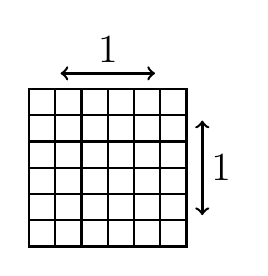
\begin{tikzpicture}[scale=2, thick]
            % Grid
            \draw[line width=1pt] (0,0) rectangle (1,1);
            \foreach \x in {1/6, 2/6, 3/6, 4/6, 5/6}
                \draw[line width=0.8pt] (\x,0) -- (\x,1);
            \foreach \y in {1/6, 2/6, 3/6, 4/6, 5/6}
                \draw[line width=0.8pt] (0,\y) -- (1,\y);
            % Horizontal arrow + 1
            \draw[<->, line width=0.9pt] (0.2,1.1) -- (0.8,1.1);
            \node at (0.5,1.25) {\Large $1$};
            % Vertical arrow + 1
            \draw[<->, line width=0.9pt] (1.1,0.2) -- (1.1,0.8);
            \node at (1.22,0.5) {\Large $1$};
        \end{tikzpicture}
        \end{center}
        mit $m$ Knoten und Gitterabstand $h=\tfrac{1}{m-1}$. Die gesamte Knotenzahl ist $n=m^2$. \\
        Die Ableitung von $f$ an der Stelle $x_0$ sei definiert durch
        \[f'(x_0) := 
        \lim_{\Delta x \rightarrow 0} \dfrac{f(x_0+\Delta x)-f(x_0)}{(x_0+\Delta x) - x_0} 
        = \lim_{\Delta x \rightarrow 0} \dfrac{f(x_0+\Delta x)-f(x_0)}{\Delta x} \]
        durch Linearisierung (Tangentengleichung) bzw. für genauere Approximationen Taylorformel ergibt sich:
        \begin{align*}
            f_L(x) &= f(x_0) + f'(x_0)(x-x_0) \\
            f(x) &= f(x_0) + f'(x_0)(x-x_0) + \tfrac{1}{2} f''(x_0)(x-x_0)^2 + \dotsc + R_n(x,x_0)
        \end{align*}
        und damit 
        \begin{align*}
            f(x+\Delta x) &= f(x_0) + f'(x_0)\Delta x + \tfrac{1}{2}f''(x_0)(\Delta x)^2 + R \tag{1}\\
            f(x-\Delta x) &= f(x_0) - f'(x_0)\Delta x + \tfrac{1}{2}f''(x_0)(\Delta x)^2 + \tilde{R} \tag{2} \\
        \end{align*}
        Mit dieser Approximation ergibt sich für die Differenzquotienten:
        \begin{align*}
            \dfrac{\diff^+}{\diff x} f(x)\mid_{x=x_0} &= \dfrac{1}{\Delta x}\left(f(x_0+\Delta x) - f(x_0)\right) 
            \tag{rechtsseitiger DQ}\\
            \dfrac{\diff^-}{\diff x} f(x)\mid_{x=x_0} &= \dfrac{1}{\Delta x}\left(f(x_0)-f(x_0+\Delta x)\right) 
            \tag{linksseitiger DQ}\\
            \dfrac{\diff}{\diff x} f(x)\mid_{x=x_0} 
            &= \dfrac{1}{2\Delta x}\left(f(x_0+\Delta x) - f(x_0-\Delta x)\right)\tag{zentraler DQ}
        \end{align*}
        Der zentrale Differenzquotienten approximiert dabei mit einer Ordnung häher als der links- und rechtsseitige 
        Differenzquotient, da quadratische Terme in (1) und (2) sich gegenseitig wegkürzen. \\ \\
        Wir nutzen dies nun um die Laplace-Operator in 2 Dimensionen zu approximieren: \\
        \begin{center}
\begin{tikzpicture}[scale=0.5, thick, every node/.style={font=\large}]

  % Gitter zeichnen
  \draw[line width=1pt] (0,0) grid (6,6);

  % Zentrum
  \def\x{3}
  \def\y{3}

  % Nachbarn markieren (blau)
  \foreach \dx/\dy in {1/0, -1/0, 0/1, 0/-1}
    \fill[mydarkblue] (\x+\dx,\y+\dy) circle (4pt);

  % Zentrumspunkt (rot)
  \fill[mydarkred] (\x,\y) circle (4pt);

  % Labels - rechts
  \node (toplabel)   [mydarkblue] at (\x+5,\y+1.5) {$(x, y{+}h)$};
  \node (centerlabel)[mydarkred]  at (\x+4.6,\y+0.5)   {$(x, y)$};
  \node (rightlabel) [mydarkblue] at (\x+5,\y-0.5) {$(x{+}h, y)$};
  % Labels - links
  \node (leftlabel)  [mydarkblue]  at (\x-5,\y-0.5)   {$(x{-}h, y)$};
  \node (bottomlabel)[mydarkblue] at (\x-5,\y-1.5) {$(x, y{-}h)$};

  % Pfeile 
  \draw[->, thick, mydarkblue] (toplabel.west)   to[out=180, in=45] (\x+0.2,\y+1+0.2);
  \draw[->, thick, mydarkred]  (centerlabel.west)to[out=180, in=45]  (\x+0.2,\y+0.2);
  \draw[->, thick, mydarkblue] (rightlabel.west) to[out=180, in=-45] (\x+1+0.2,\y-0.2);
  \draw[->, thick, mydarkblue] (leftlabel.east) to[out=0, in=-135] (\x-1-0.2,\y-0.2);
  \draw[->, thick, mydarkblue] (bottomlabel.east) to[out=0, in=-135] (\x-0.2,\y-1-0.2);

\end{tikzpicture}
        \end{center}
        Für innnere Punkte in unserem Quadratgitter gilt die sogenannte \glqq 5-Punktregel\grqq{}:
        \[-h^{-2}\left(u(x+h,y)-2u(x,y)+u(x-h,y)+u(x,y+h)-2u(x,y)+u(x,y-h)\right)=f(x,y)\]
        Durch Berücksichtigung der Randbedingung $u(x,y)=0$ für $(x,y)\in\partial Q$ ist dies äquivalent zu einem 
        linearen Gleichungssystem $Ax=b$ für den Vektor $x\in\mathbb{R}^n$ der unbekannten Knotenwerte 
        $x_i=u(P_i)$
        Die Matrix $A$ hat die Gestalt
        \[A = \left.\begin{pmatrix}
            B & -I & 0 & \dots\\
            -I & B & -I & \\
            0 & -I & B & \ddots \\
            \vdots& & \ddots & \ddots
        \end{pmatrix}\right\} n \quad \text{ mit } B = \left.\begin{pmatrix}
            4 & -1 & 0 & \dots\\
            -1 & 4 & -1 & \\
            0 & -1 & 4 & \ddots \\
            \vdots& & \ddots & \ddots
        \end{pmatrix}\right\}m\]
        und der Einheitsmatrix $I$, d.h. $B,I\in\mathbb{R}^{m\times m}$. 
        Die rechte Seite ist $b=h^2(f(P_1),\dotsc,f(P_n))^T$. \\
        Wir erhalten ein sehr großes LGS mit dünn besetzter Bandmatrix mit Bandbreite $2m+1$, symmetrisch, 
        schwach diagonaldominant, positiv definit. Es biete sich also an unsere iterativen Verfahren zum Lösen 
        anzuwenden.
    \end{egbox}
    \newpage
    \subsubsection{Konvergenzgeschwindigkeit des CG-Verfahren}
    \begin{thmbox}{Satz}[CG-Konvergenz]
        Sei $x$ die Lösung des linearen Gleichungssystems $Ax=b$. Für das CG-Verfahren gilt die Fehlerabschätzung
        \[\|x^{(k)} - x\|_A \leq 2\left(\dfrac{\sqrt{\kappa(A)-1}}{\sqrt{\kappa}}+1\right)^k \cdot \|x^{(0)}-x\|\]
        Zur Reduktion des Anfangsfehlers um den Faktor $\varepsilon$ sind circa 
        \[k(\varepsilon)\approx \tfrac{1}{2}\sqrt{\kappa(A)}\cdot \ln(\tfrac{2}{\varepsilon}) +1 \]
        Iterationsschritte erforderlich. 
    \end{thmbox}
    Für den Beweis des Satzes benötigen wir noch einen Hilfssatz:
    \begin{thmbox}{Hilfssatz}[polynomiale Normschranke]
        Für ein Polynom $p\in P_k:=\mathbb{R}_k[X]$ mit $p(0)=1$, gelte auf einer Menge $S\subset \mathbb{R}$, welche
        alle Eigenwerte von $A$ enthält, $\sup_{\mu\in S} |p(\mu)| \leq M$. Dann gilt 
        \[\|x^{(k)} - x\|_A \leq M\cdot\|x^{(0)}-x\|_A\]
    \end{thmbox}
    \textit{Beweis des Hilfssatz.} Unter Beachtung der Beziehung 
    \[\|x^{(k)}-x\|_A = \min\{\|y-x\|_A : y\in x^{(0)}+\mathcal{K}_k(A,r^{(0)})\}\]
    erhalten wir 
    \[\|x^{(k)}-x\|_A = \min_{p\in P_{k-1}}\|x^{(0)}-x+p(A)r^{(0)}\|_A\]
    Wegen $r^{(0)} = Ax^{(0)}-b = A(x^{(0)}-x)$ folgt
    \begin{align*}
        \|x^{(k)}-x\|_A &= \min_{p\in P_{k-1}} \|(I+A\cdot p(A))\cdot (x^{(0)}-x)\|_A \\
        &\leq \min_{p\in P_{k-1}} \|I+A\cdot p(A)\|_A\cdot\|x^{(0)}-x\|_A \\
        &\leq \min_{p\in P_{k-1}, p(0)=1} \|p(A)\|_A\cdot\|x^{(0)}-x\|_A 
    \end{align*}
    mit der von $A$-Norm (Energienorm)$\|\cdot\|_A$ erzeugten natürlichen Matrixnorm $\|\cdot\|_A$. \\
    Für beliebiges $y\in\mathbb{R}^n$ gilt mit einer Orthonormalbasis $\{w_1,\dotsc,w_n\}$ aus Eigenvektoren von $A$:
    \[y=\sum_{j=1}^{n}\gamma_j w_j,\quad \gamma_j = \langle y, w_j\rangle\]
    und folglich 
    \[\|p(A)y\|_A^2 = \sum_{j=1}^{n} \lambda_j p(\lambda_j)^2\gamma_j^2 
    \leq M^2 \sum_{j=1}^{n} \lambda_j \gamma_j^2 = M^2 \|y\|_A^2\]
    Dies impliziert 
    \[\|p(A)\|_A = \sup_{y\in\mathbb{R}^n\backslash\{0\}} \dfrac{\|p(A)y\|_A}{\|y\|_A}\leq M\]
    und damit die Behauptung. \qed \\ \\
    \textit{Beweis von Satz 2.21}Durch Verwendung des Hilfssatz mit $S:=[\lambda, \Lambda]$, 
    wobei $\lambda$ den kleinsten un d$\Lambda$ den größten Eigenwert von $A$ beschreibt, folgt:
    \[\|x^{(k)}-x\|_A \leq \min_{p\in P_{k-1}, p(0)=1} 
    \left(\sup_{\lambda\leq\mu\leq\Lambda}|p(\mu)|\right)\cdot\|x^{(0)}-x\|_A \]
    Dies ergibt die Behauptung wenn wir noch zeigen können, dass 
    \[\sup_{\lambda\leq\mu\leq\Lambda}|p(\mu)| 
    \leq 2\cdot \dfrac{(1-\sqrt{\tfrac{\lambda}{\Lambda}})^k}{(1+\sqrt{\tfrac{\lambda}{\Lambda}})^k}\]
    Hierbei handelt es sich um ein Problem der Bestapproximation von Polynomen bzgl. 
    der Maximumsnorm (Chebyshev-Approximation).
    Die Lösung $\overline{p}$ ist gegeben durch 
    \[\overline{p}(\mu) = \dfrac{T_k(\tfrac{\Lambda+\lambda-2\mu}{\Lambda-\lambda})}
    {T_k(\tfrac{\Lambda+\lambda}{\Lambda-\lambda})},\]
    wobei $T_k$ das $k$-te Chebyshev-Polynom auf $[-1,1]$ ist. Es folgt
    \[\sup_{\lambda\leq\mu\Lambda} = T_k\left(\dfrac{\Lambda+\lambda}{\lambda-\lambda}\right)^{-1}\]
    Aus der Darstellungen
    \[T_k(\mu) = \tfrac{1}{2}\left((\mu+\sqrt{\mu^2-1})^k+(\mu-\sqrt{\mu^2-1})^k\right), 
    \quad \text{für } \mu\in[-1,1]\]
    für die Chebyshev-Polynome folgt mittels der Identität
    \[\dfrac{\kappa+1}{\kappa-1} + \sqrt{\left(\dfrac{\kappa+1}{\kappa-1}\right)^2-1} 
    = \dfrac{\kappa+1}{\kappa-1} + \dfrac{2\sqrt{\kappa}}{\kappa-1} = \dfrac{(\sqrt{\kappa}+1)^2}{\kappa - 1}
    = \dfrac{\sqrt{\kappa}+1}{\sqrt{\kappa}-1}\]
    die folgende Abschätzung nach unten:
    \[T_k\left(\dfrac{\Lambda+\lambda}{\Lambda-\lambda}\right) = T_k\left(\dfrac{\kappa+1}{\kappa-1}\right)
    = \dfrac{1}{2}\left(\left(\dfrac{\sqrt{\kappa}+1}{\sqrt{\kappa}-1}\right)^k + 
    \left(\dfrac{\sqrt{\kappa}-1}{\sqrt{\kappa}+1}\right)^k\right) 
    \geq \left(\dfrac{\sqrt{\kappa}+1}{\sqrt{\kappa}-1}\right)^k\]
    Also wird $\sup_{\lambda\leq\mu\leq\Lambda}\overline{p}(\mu)
    \leq 2\left(\tfrac{\sqrt{\kappa}-1}{\sqrt{\kappa}-1}\right)^k$, was die erste Ungleichung des Satzes zeigt. \\
    Für den zweiten Teil betrachten wir die Anzahl der Schritte, dass
    \[2\left(\dfrac{\sqrt{\kappa}-1}{\sqrt{\kappa}-1}\right)^{k(\varepsilon)} < \varepsilon \quad \iff \quad 
    k(\varepsilon) > \ln(\tfrac{2}{\varepsilon})\cdot
    \left(\ln\left(\dfrac{\sqrt{\kappa}-1}{\sqrt{\kappa}-1}\right)\right)^{-1}\]
    Wegen der Reihendarstellung $\ln\tfrac{x+1}{x-1} = 2(\tfrac{1}{x} + \tfrac{1}{3}\tfrac{1}{x^3} 
    + \tfrac{1}{5}\tfrac{1}{x^5} + \dotsc)$ ist die zweite Ungleichung genau dann erfüllt wenn 
    \[k(\varepsilon) > \tfrac{1}{2}\sqrt{\kappa}\ln(\tfrac{2}{\varepsilon})\]
    \qed